
\section{Динамика выбросов загрязняющих веществ}
\begin{frame}{\insertsectionhead}
    \begin{center}
        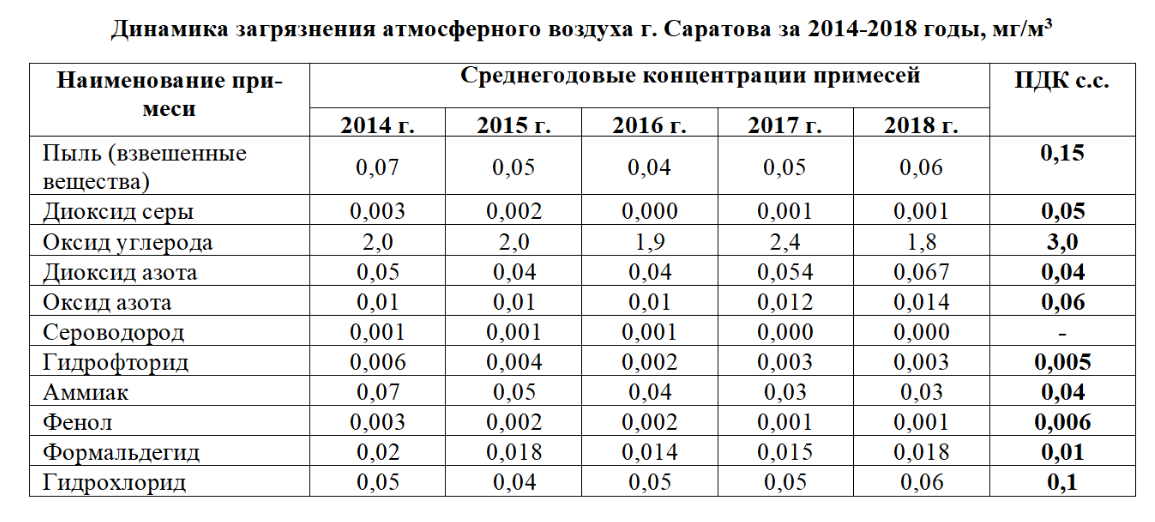
\includegraphics[width=0.75\textwidth]{assets/tendations.png}
    \end{center}

    Как видно из таблицы в Саратове концентрация пыли, диоксида серы, оксидов азота,
    формальдегида, гидрофторида и гидрохлорида 
    имеют тенденцию к росту.
\end{frame}

\begin{frame}{\insertsectionhead}
    \begin{center}
        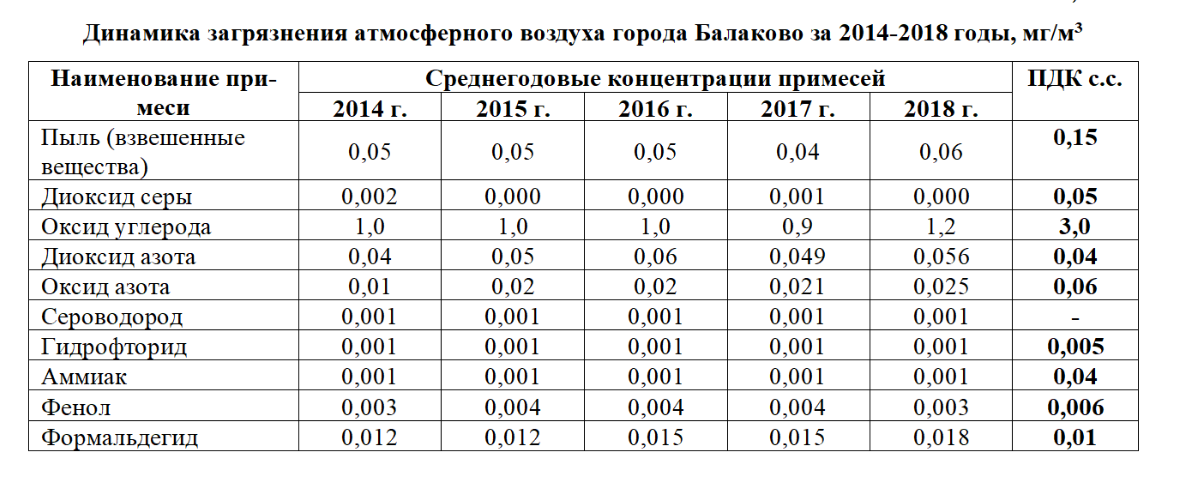
\includegraphics[width=0.75\textwidth]{assets/balakovo.png}
    \end{center}

    Как видно из таблицы в городе Балаково концентрация пыли, оксидов азота и
    формальдегида имеют тенденцию к росту.
\end{frame}

